\pagestyle{chapter-fancy-style}
\chapter{Software design}

%=====================
\section{Overview}
The ROV software can be split into two distinct parts - the code present on the Arduino, which translates the operator commands to physical actions of the vehicle, as well as the shore-based computer part, which collects the user inputs and sends the corresponding commands to the Arduino. The remainder of this chapter covers both parts of the software separately. The computer part of the code is intended as cross-platform because its based on Python~2.7 and its open-source libraries. However, it has been developed and tested exclusively on Ubuntu 12 and 14.

%=====================
\section{Micro-controller}

%---------------------
\subsection{Program structure}
The Arduino only receives and executes operator commands, which means its functional flow is rather simple, as shown in the flowchart in Fig.~\ref{fig:arduinoMainLoop}. The \texttt{execute every instruction in series block} might involve arming the ESCs, sending readings of all the sensors, switching the forward LEDs on or off, and setting thrust levels and directions of all the motors.

\begin{figure}[]
\centering
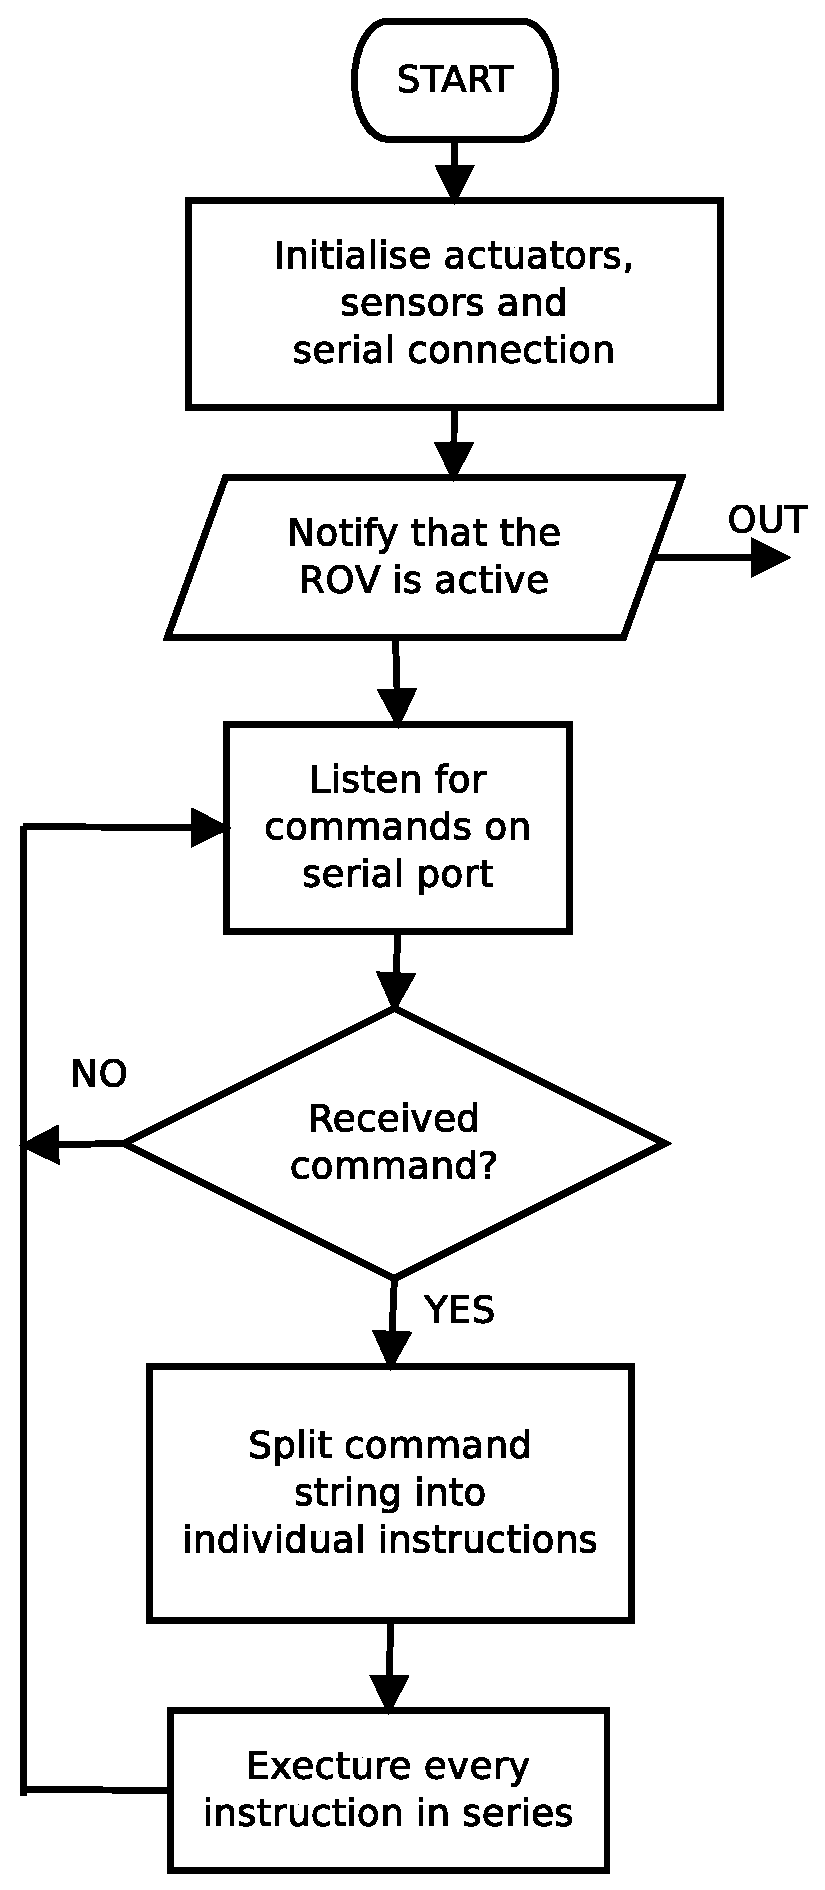
\includegraphics[width=0.4\linewidth]{arduinoSWFlowchart.eps}
\caption{Block diagram showing the flow of the Arduino \texttt{setup()} and \texttt{loop()} functions.}
\label{fig:arduinoMainLoop}
\end{figure}

%---------------------
\subsection{Hardware interfaces}
In order to interact with each piece of hardware, such as a sensor or electric motor, or in order to implement simple functionality, a special class \texttt{Module} has been implemented. This is holds fields such as \texttt{identifier} and \texttt{currentValue}, the combination of which is used to control a single aspect of the Arduino operation. For example, a~\texttt{Module} object called \texttt{refreshRate} holds the loop frequency the micro-controller operates at. Such basic objects typically get used directly in the \texttt{loop()} method and are treated as simple storage containers. For instance, at the end of each \texttt{loop()} call a new delay gets set as \texttt{delay(refreshRate.getValue());}, which allows setting the delay value using the same command protocol as used with more complex \texttt{Module}s.

Key methods of the \texttt{Module} class are the virtual \texttt{getValue()}, \texttt{setValue(int newValue)}, and \texttt{arm()} functions. Their default implementation in the \texttt{Module} class allows the user to read or set the value the object holds, for instance the refresh rate of the Arduino, or to initialise the object at the beginning of the execution.

Each of the modules gets created upon initialisation of the Arduino code and pointers to them are collected in arrays \texttt{Module* actuators[]} or \texttt{Module* sensors[]}, depending on their functionality. This arrangement allows the user to create classes derived from \texttt{Module} and overriding the functionality they execute when given or asked for a new value, at the same time allowing the same code in the main program loop to be used to interact with each object. A depiction of the currently used classes is shown in Figure \ref{fig:moduleClasses}. This approach is used primarily in the \texttt{parseInput()} method which is responsible for communication between the micro-controller and the PC or the \texttt{sendSensorReadings()} method which calls the \texttt{getValue()} function on each sensor module and encodes their readings into a string message which gets sent to the PC.

Currently implemented classes derived from \texttt{Module} are:
%
\begin{itemize}
\item \texttt{BrushlessDCMotor} - accepts negative and positive demand on the motor rps into the \texttt{setValue} function, treating negative values as reverse. Uses two assigned output pins in order to control the direction (binary digital output) and speed (PWM) of the motor via the ESC.
\item \texttt{LEDModule} - the value passed to the \texttt{setValue} method is treated as a binary switch telling the module to set the output pin either to HIGH or LOW state, thus controlling the LED.
\item \texttt{DepthSensor} - implements the \texttt{getValue()} method in order to return the current depth. Currently, this is a~\textbf{placeholder only}.
\end{itemize}

\begin{figure}[p]
\centering
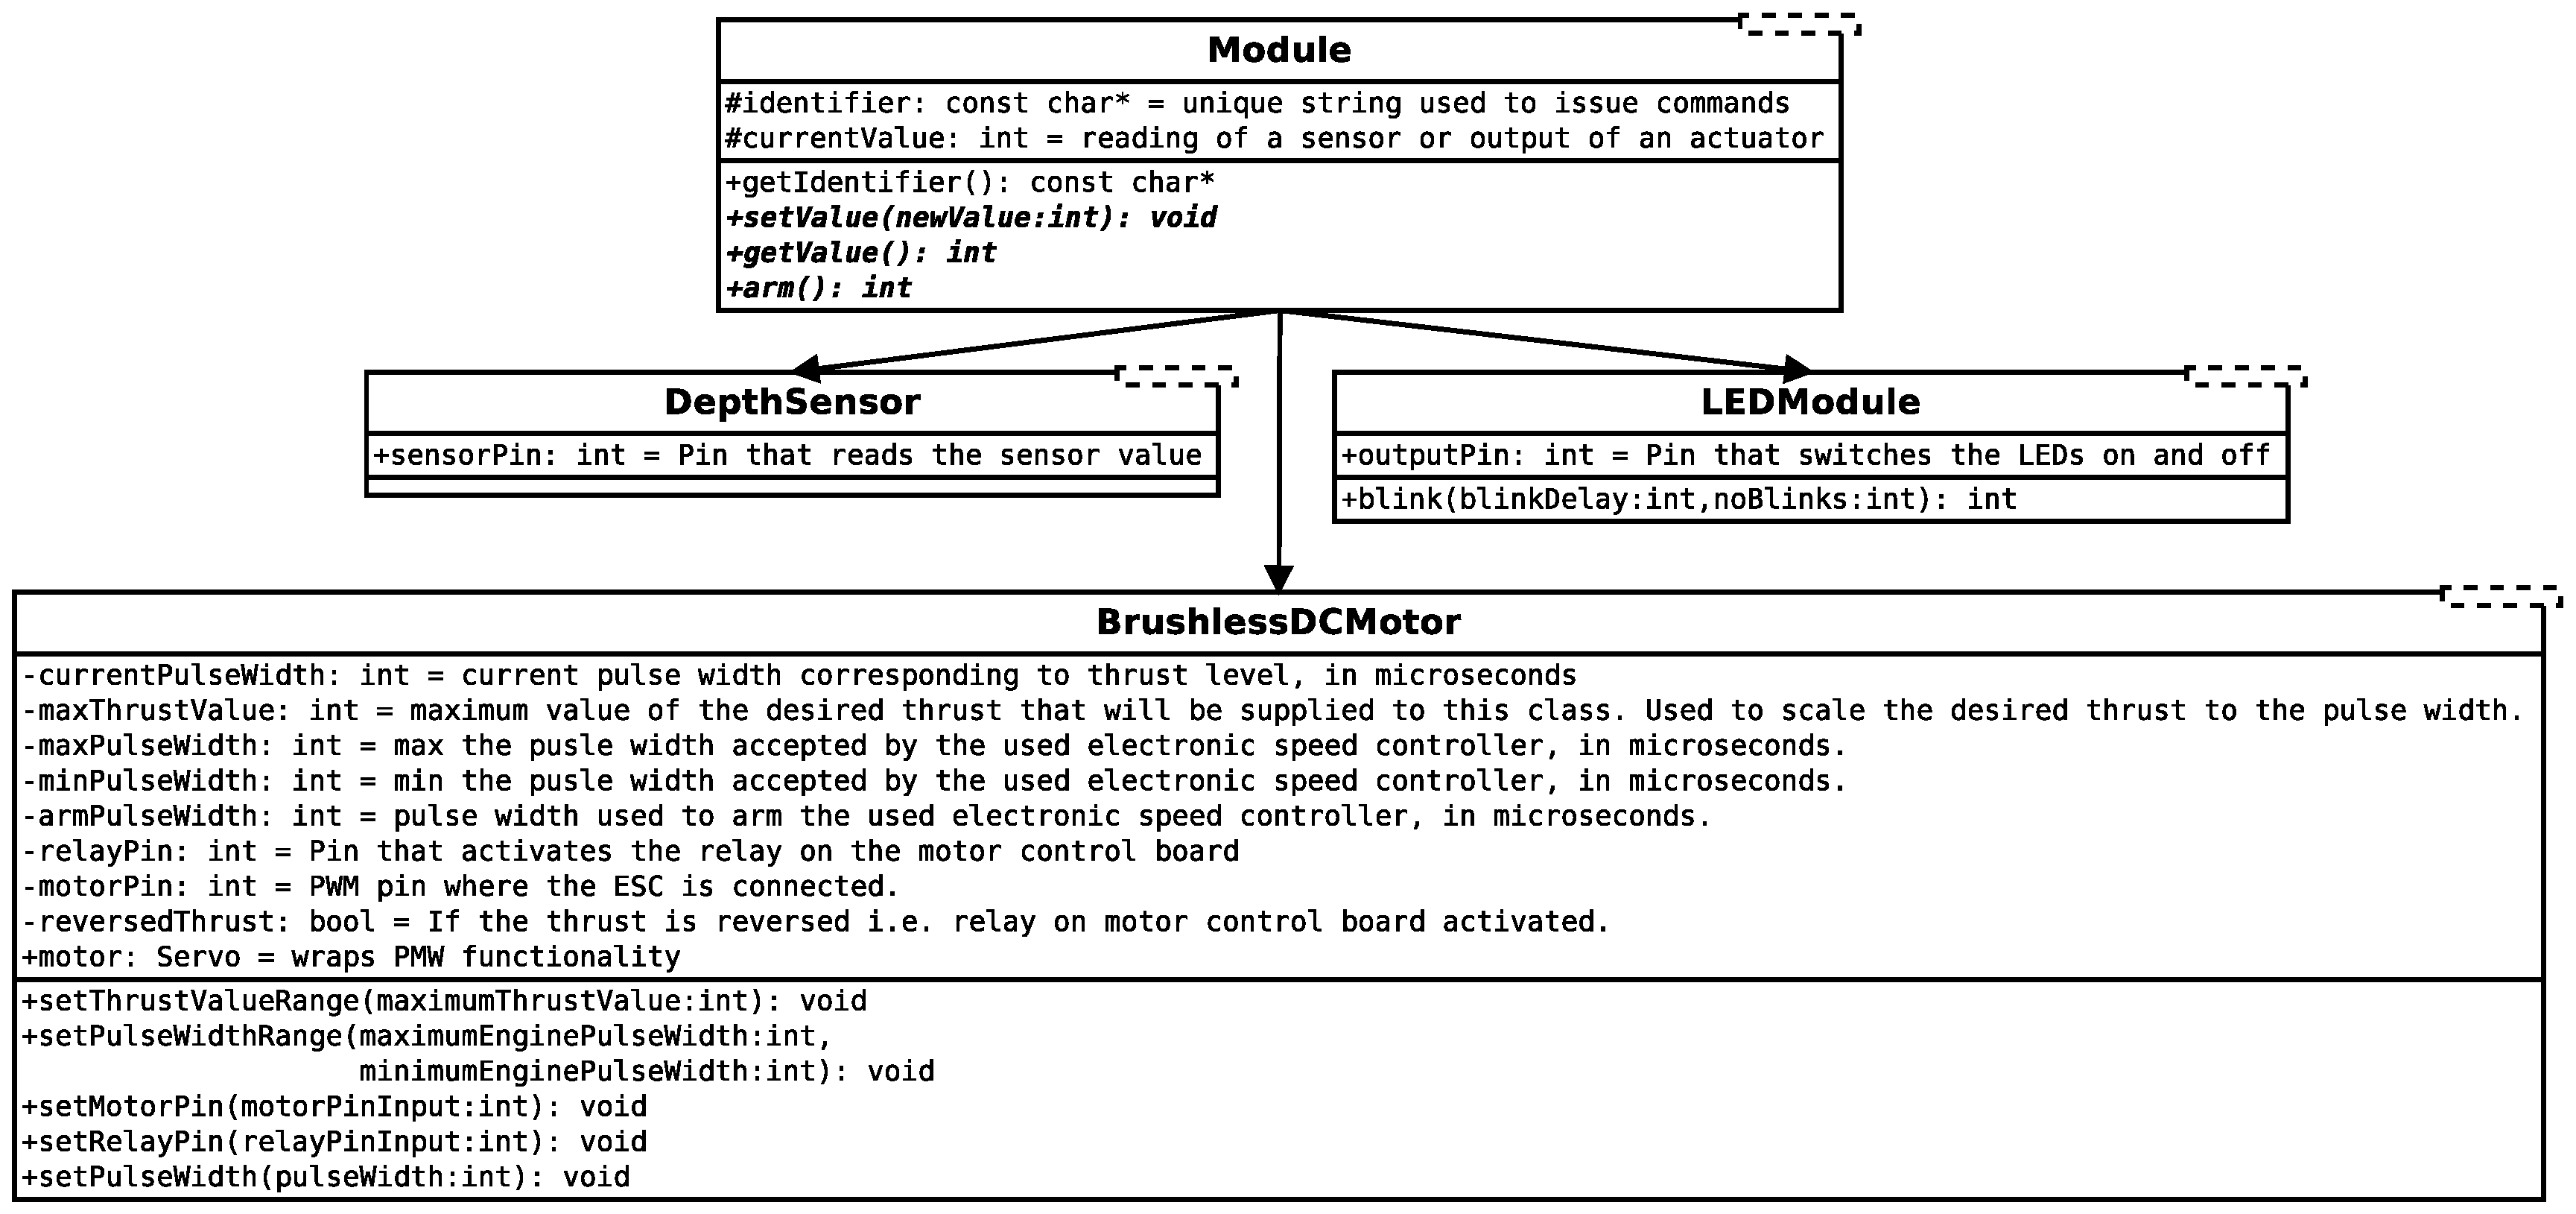
\includegraphics[width=0.8\textheight,angle=90]{ardunioSWClassDiagram.eps}
\caption{Block diagram showing the class hierarchy of the \texttt{Module} classes used to control Arduino functionality.}
\label{fig:moduleClasses}
\end{figure}

%---------------------
\subsection{Communications}

The ROV communicates with the computer via a serial port using the USB connection. The process involves encoding messages into one-line strings and dumping them into the buffer for the other side to see. This imposes a need for strict formatting of the message packets, which is described in Table \ref{tab:commsEncoding}. Each message consists of a string flag denoting an action or a subsystem, for instance "forwardLED" or "sendSensorReadings", followed by an integer value. An arbitrary number of commands may be sent in any one packet although the length of the entire message is limited by the character buffer size on the Arduino.

During each loop, the micro-controller attempts to read data from the serial port. If any data is found, the \texttt{parseInput()} method gets called. This is responsible for checking whether the passed information conforms to the message encoding system. If yes, the string gets unwrapped into a series of flags and corresponding values. Certain flags do not require the value and so an arbitrary integer may be passed, typically a 1 indicating a boolean true.

Each flag is then compared to the names of the registered \texttt{Module} objects until a match has been found. The value corresponding to the flag gets then passed using the virtual \texttt{setValue(int value)}. This is implemented by each class derived from the baseline \texttt{Module} class if a special action is required when a new value gets passed. For instance, the \texttt{BrushlessDCMotor} class converts the integer throttle demand into values understood by the ESC and adjusts the PWM signal, flipping the thrust direction relay if necessary. Other modules holding simple integer or boolean values do not re-implement the \texttt{setValue} method.

\begin{table}[h]
\centering
\caption{Description of the special characters used to format string messages sent over the serial port.}
\label{tab:commsEncoding}
\begin{tabular}{@{}ll@{}}
\toprule
\textbf{Character} & \textbf{Meaning} \\ \midrule
$<$ & beginning of message to PC \\
$>$ & beginning of message to Arduino \\
, & delimiter \\
; & end of message \\
\bottomrule
\end{tabular}
\end{table}

%=====================
\section{Computer}

%---------------------
\subsection{Program structure}
The key piece of code that runs as an executable is the \texttt{ROVgui.py}. It
defines a class \texttt{rovGuiMainFrame}, which then gets executed inside~a 
wxWidgets application. The class itself is derived from a~base class, which
defines the basic functionality of the graphical user interface alone (discussed
in more detail later) but all of the code responsible for the operation of the
ROV itself is contained in \texttt{ROVgui.py}.
The class contains several timers which execute specific methods at fixed intervals,
for instance they ask the mirco-controller to send the sensor readings or pass
demands for the electric motors.
Each of the key aspects of the code will be discussed in more detail in the following
parts of this chapter.

%---------------------
\subsection{Communications}
The protocol used to communicate with the micro-controller via the serial connection
utilises the \texttt{serial} Python library. This simply opens a port and treats
it as a buffer to read and write from. All of the parsed messages adhere to the
structure used by the Arduino side, namely begin and end with specific characters
and each element is separated by a known delimiter. The following code listing
provides a minimum example showing how a known port is opened, written into and
read from.

\begin{lstlisting}[style=myPythonStyle,language=Python]
import serial
import time

BAUD_RATE = 19200
REFRESH_RATE = 100
PORT = "/dev/ttyACM0"

# open the connection
serialConnection = serial.Serial(PORT, BAUD_RATE, timeout = 2)

testMsgGood = True
try:
    serialConnection.inWaiting()
except:
    testMsgGood = False

if not serialConnection or not serialConnection.readable() or not testMsgGood:
    raise IOError("Connection is FUBAR!")

# keep looping and printing whatever we get from the serial
message = ">sendSensorReadings,1;"
while True:
	serialConnection.write(message)
    line = serialConnection.readline().replace("\n","")
    if line:
        print line
    time.sleep(1./REFRESH_RATE)
\end{lstlisting}

%---------------------
\subsection{User input}
Interface to the Xbox controller (Figure \ref{fig:xboxController}) has been
created using pyGame 1.9.1, an open-source library for game development.
The interface relies on pyGame joystick module capturing all the inputs provided
by the user via the controller as events. These are stored in a buffer and then
the main GUI function periodically calls the \texttt{parseEvents()} method implemented
in the \texttt{controller} class. This retrieves the most recent set of events,
clears the buffer, and updates the values of axes and button positions held
inside the \texttt{controller} object. From here they are accessed from the main GUI each time a new
set of input parameters gets sent to the micro-controller.
A minimum working example which captures the events and prings the current axes
positions in the terminal is provided

\begin{lstlisting}[style=myPythonStyle,language=Python]
import pygame
from pygame.locals import *

pygame.init()
clock = pygame.time.Clock()

joysticks = []
for i in range(0, pygame.joystick.get_count()):
        joysticks.append(pygame.joystick.Joystick(i))
        joysticks[-1].init()
        print "Detected joystick '",joysticks[-1].get_name(),"'"
while 1:
        clock.tick(60)
        for event in pygame.event.get():
                if event.type == QUIT:
                        print "Received event 'Quit', exiting."
                        return
                elif event.type == KEYDOWN and event.key == K_ESCAPE:
                        print "Escape key pressed, exiting."
                        return
                elif event.type == KEYDOWN:
                        print "Keydown,",event.key
                elif event.type == KEYUP:
                        print "Keyup,",event.key
                elif event.type == MOUSEMOTION:
                        print "Mouse movement detected."
                elif event.type == MOUSEBUTTONDOWN:
                        print "Mouse button",event.button,"down at",pygame.mouse.get_pos()
                elif event.type == MOUSEBUTTONUP:
                        print "Mouse button",event.button,"up at",pygame.mouse.get_pos()
                        
                elif event.type == JOYAXISMOTION:
                        print "Joystick '",joysticks[event.joy].get_name(),"' axis",event.axis,"motion."
                        if event.axis == 2:
                                print ' axis 2', event.value
                        elif event.axis == 5:
                                print ' axis 5', event.value
                elif event.type == JOYBUTTONDOWN:
                        print ("Joystick '",joysticks[event.joy].get_name(),
                            "' button",event.button,"down.")
                elif event.type == JOYBUTTONUP:
                        print "Joystick '",joysticks[event.joy].get_name(),"' button",event.button,"up."
                elif event.type == JOYHATMOTION:
                        print "Joystick '",joysticks[event.joy].get_name(),"' hat",event.hat," moved to",event.value
\end{lstlisting}

\begin{figure}[]
\begin{center}
\includegraphics*[width=0.6\textwidth,angle=0]{xboxController.jpg}
\end{center}
\caption{USB Xbox controller used to provide control inputs to the ROV.}
\label{fig:xboxController}
\end{figure}

%---------------------
\subsection{Video acquisition}

In order to acquire imagery from the on-board USB camera, the code uses OpenCV 3.0.0-rc1,
a cross-platform, open-source digital imaging library. It is written in C++ but
provides a straightforward interface for use in Python.
In short, capturing a single frame is achieved as

\begin{lstlisting}[style=myPythonStyle,language=Python]
import cv2, wx
# create a camera
cameraID = 1
cameraCapture = cv2.VideoCapture(cameraID)
# get a picture and set up colours
ret, picture = cameraCapture.read()
height, width = picture.shape[:2]
picture = cv2.cvtColor(picture, cv2.COLOR_BGR2RGB)
# convert to wxWidgets bitmap for use inside the GUI
bmp = wx.BitmapFromBuffer(width, height, picture)
\end{lstlisting}

%---------------------
\subsection{Graphical interface}

Figure \ref{fig:GUI} shows the layout used to provide a graphical interface for
controlling the ROV. Live feed from the on-board camera is provided on the right-hand
side while the left is devoted to controlling the top-level functionality of the
vehicle. The top left-hand corner shows the thruster demand of each motor. Below,
controls are provided for the serial port connection to the Arduino, the video
feed of the camera, Xbox controller and arming of the electronic speed controllers
on board of the ROV.
There is also a pop-up Settings window which allows the user to adjust the
Arduino loop frequency, as well as frequencies for sending the control inputs,
receiving sensor readings, and camera frame rate.
The entire GUI runs on wxWidgets 2.8.12.1 and has been designed using wxFormBuilder,
both of which may be readily integrated with Python and are open-source.

\begin{figure}[]
\begin{center}
\includegraphics*[width=0.8\textwidth,angle=0]{GUI.png}
\end{center}
\caption{Graphical user interface (GUI) used to control the ROV from the laptop.}
\label{fig:GUI}
\end{figure}
